\section{Correlations and the dynamic structure factor}\label{sec:4.2}

A dark-matter particle in silicon scatters at a rate fixed by the dynamic structure factor $S(\vect{q},\omega)$ of \cref{eq:2.5-golden}, which counts the transitions the target makes. A weak potential applied from outside, acting through the same density operator (\cref{sec:4.1}), makes the density ripple by an amount fixed by the response function $R_{ee}$ of \cref{eq:4.1-kubo}. Both are built from the same matrix elements and the same Gibbs weights, and we will see that at each $\vect{q}$ and $\omega$ either one fixes the other. This is the fluctuation--dissipation theorem, and it lets every method that computes a response also compute a rate. Before we get there, we look at $S$ from two other sides. In space and time it is the Fourier transform of a density--density correlation function, Van Hove's picture of a scattering experiment. Over several target operators it is a positive matrix, which keeps every rate positive and bounds the interference between two couplings. We end with independent particles, for which $S$ has a closed form in the electron gas, and the hydrogen atom of \cref{sec:2.2} comes back as a special case. The treatment follows Refs.~\cite[Chaps.~3 and 4]{giuliani2005quantum} and \cite[Chap.~2]{pines1966theory}.

\subsection{The response matrix}

A dark photon couples to the charge of the electrons and of the nuclei, with opposite signs, and other mediators couple to spin or to the nucleon number (\cref{sec:1.4}). In general the interaction between the dark-matter plane waves $\vect{p}$ and $\vect{p} - \vect{q}$ is a sum $\Vol^{-1}\sum_b\tilde V_b(\vect{q})\,O_b(\vect{q})$ over target operators $O_b(\vect{q})$, each with its own potential $\tilde V_b(\vect{q})$; the density coupling of \cref{eq:A.3-vertex} is the case of a single term, $O_e = n_e(\vect{q})$ with $\tilde V_e = \tilde V$. The golden-rule amplitude to reach $|f\rangle$ from $|i\rangle$ is then $\Vol^{-1}\sum_b\tilde V_b\langle f|O_b|i\rangle$. Its square has cross terms $\tilde V_a^*\tilde V_b\,\langle i|O_a^\dagger|f\rangle\langle f|O_b|i\rangle$, and the target enters through the matrix of their thermal sums.
\begin{keyresult}[Response matrix]
\begin{equation}
  \begin{aligned}
  S_{ab}(\vect{q},\omega) &= \frac{2\pi}{\Vol}\sum_{i,f}p_i\,\langle i|O_a(\vect{q})^\dagger|f\rangle\langle f|O_b(\vect{q})|i\rangle\,\delta(\omega - E_f + E_i) \\
  &= \frac{1}{\Vol}\int_{-\infty}^{\infty}\dd t\;\ee^{\ii\omega t}\,\bigl\langle O_a(\vect{q},t)^\dagger\,O_b(\vect{q},0)\bigr\rangle .
  \end{aligned}
  \label{eq:4.2-Sab}
\end{equation}
Its diagonal elements are the transition sums of \cref{eq:2.5-transum}, $S_{aa} = (2\pi/\Vol)\,\mathcal{S}_{O_a}$, and the dynamic structure factor is the density element, $S \equiv S_{ee}$.
\end{keyresult}
The correlation-function form follows as \cref{eq:2.5-corr} did. Inserting a complete set of states between the two operators, each term oscillates as $\ee^{-\ii(E_f - E_i)t}$, and the time integral turns the oscillation into $2\pi\,\delta(\omega - E_f + E_i)$. This is the definition \cref{eq:A.7-S}, and its density element is $S(\vect{q},\omega)$ of \cref{eq:2.5-golden}, Ref.~\cite[Eq.~(4)]{knapen2021dark}, with the same normalization. Exchanging $a$ and $b$ complex-conjugates each term, so $S_{ab}^* = S_{ba}$ and the matrix is Hermitian. Like $R_{ab}$, it is intensive, and for density operators it has the dimension $\mathrm{eV}^2$. Detailed balance carries over with the indices exchanged. For operators with $O(-\vect{q}) = O(\vect{q})^\dagger$, relabeling $i \leftrightarrow f$ as in \cref{eq:2.5-db} gives $S_{ab}(-\vect{q},-\omega) = \ee^{-\beta\omega}S_{ba}(\vect{q},\omega)$, which is \cref{eq:A.7-DB}.

The sum over final dark-matter momenta is the one of \cref{sec:2.5}, term by term, and the rate per dark-matter particle is
\begin{equation}
  \varGamma = \int\frac{\dd^3q}{(2\pi)^3}\sum_{a,b}\tilde V_a(\vect{q})^*\,\tilde V_b(\vect{q})\,S_{ab}(\vect{q},\omega_{\vect{q}}) ,
  \label{eq:4.2-rate}
\end{equation}
with $\omega_{\vect{q}}$ the energy deposited at $\vect{q}$ (\cref{sec:2.5}). For a single operator it reduces to $\int\dd^3q\,(2\pi)^{-3}|\tilde V_a|^2S_{aa}$, and for the density to \cref{eq:2.5-golden}. The off-diagonal elements carry the interference between two couplings. For a dark photon, for instance, the electron and nuclear densities enter with potentials of opposite sign, and $S_{ab}$ between them measures how the electrons follow a recoiling nucleus; \cref{chap:8} builds the general rate on \cref{eq:4.2-rate}.

\subsection{Correlations in space and time}

At a typical momentum transfer $q_0 = \alpha m_e = \SI{3.73}{keV}$ the dark matter probes the electron density on a length $2\pi/q_0 = \SI{3.32}{\angstrom}$, and at an energy of \SI{10}{eV} over a time $1/\omega = \SI{0.066}{fs}$. The structure factor can be read as a statement about the density on these scales. Van Hove introduced this reading for neutron scattering~\cite{vanhove1954correlations}: the rate measures how the density at one place and time is correlated with the density at another. To see it, write the density in position space, $\op{\nd}_e(\vect{r}) = \sum_j\delta^3(\vect{r} - \vect{r}_j)$, the operator whose transform \cref{eq:A.3-space} is $n_e(\vect{q})$, and define the Van Hove correlation function
\begin{equation}
  \mathcal{G}_{\mathrm{VH}}(\vect{r},t) = \frac{1}{N_e}\int\dd^3r'\,\bigl\langle\op{\nd}_e(\vect{r}',0)\,\op{\nd}_e(\vect{r}' + \vect{r},t)\bigr\rangle ,
  \label{eq:4.2-GVH}
\end{equation}
with $N_e$ the number of electrons in the volume $\Vol$ and the Heisenberg operators of \cref{sec:4.1}. In the correlation form \cref{eq:4.2-Sab}, stationarity moves the time from one operator to the other, $\langle n_e(\vect{q},t)^\dagger n_e(\vect{q},0)\rangle = \langle n_e(\vect{q},0)^\dagger n_e(\vect{q},-t)\rangle$. Writing both operators as integrals over position, $n_e(\vect{q})^\dagger = \int\dd^3r'\,\ee^{-\ii\vect{q}\cdot\vect{r}'}\op{\nd}_e(\vect{r}')$, and writing the position in $n_e(\vect{q},-t)$ as $\vect{r}' + \vect{r}$,
\begin{equation*}
  \begin{aligned}
  \langle n_e(\vect{q},0)^\dagger n_e(\vect{q},-t)\rangle &= \int\dd^3r\;\ee^{\ii\vect{q}\cdot\vect{r}}\int\dd^3r'\,\bigl\langle\op{\nd}_e(\vect{r}',0)\,\op{\nd}_e(\vect{r}'+\vect{r},-t)\bigr\rangle \\
  &= N_e\int\dd^3r\;\ee^{\ii\vect{q}\cdot\vect{r}}\,\mathcal{G}_{\mathrm{VH}}(\vect{r},-t) .
  \end{aligned}
\end{equation*}
Dividing by $\Vol$, integrating over $t$ with $\ee^{\ii\omega t}$ and reversing the sign of $t$,
\begin{equation}
  S(\vect{q},\omega) = \nd_e\int_{-\infty}^{\infty}\dd t\int\dd^3r\;\ee^{\ii(\vect{q}\cdot\vect{r} - \omega t)}\,\mathcal{G}_{\mathrm{VH}}(\vect{r},t) ,
  \label{eq:4.2-vanhove}
\end{equation}
with $\nd_e = N_e/\Vol$. The dynamic structure factor is the space--time Fourier transform of the Van Hove function, per unit volume. Inserted into \cref{eq:2.5-golden}, this is the Born rate of any target written through its density correlations, the form Van Hove derived for neutrons scattering on nuclei.

The classical reading of $\mathcal{G}_{\mathrm{VH}}$ is simple. For commuting densities, \cref{eq:4.2-GVH} becomes $N_e^{-1}\sum_{j,l}\langle\delta^3(\vect{r} + \vect{r}_j(0) - \vect{r}_l(t))\rangle$: given an electron at the origin at $t = 0$, it is the density of electrons at $\vect{r}$ at time $t$. The terms with $j = l$ follow the electron itself. They integrate to one and spread out as the electron moves away. The terms with $j \ne l$ describe all the others, and they tend to $\nd_e$ at large $r$. At $t = 0$ the function is $\delta^3(\vect{r}) + \nd_e\,g_{\mathrm{pair}}(\vect{r})$, with $g_{\mathrm{pair}}(\vect{r})$ the pair distribution, the probability of finding a second electron at $\vect{r}$ relative to the first, normalized to one at large separation. Quantum mechanically, however, the densities at different times do not commute, and $\mathcal{G}_{\mathrm{VH}}$ is complex for $t \ne 0$. Its imaginary part is what makes $S(\vect{q},\omega)$ and $S(-\vect{q},-\omega)$ differ by the factor $\ee^{-\beta\omega}$ of detailed balance, and it drops out when $|\omega| \ll T$.

A single free electron shows how the time dependence encodes the recoil. Take it at rest, in the plane wave $\vect{p} = 0$. Then $n_e(\vect{q},t) = \ee^{\ii Ht}\ee^{\ii\vect{q}\cdot\vect{r}}\ee^{-\ii Ht}$ acting on $|\vect{0}\rangle$ gives $\ee^{\ii q^2t/2m_e}|\vect{q}\rangle$, and the correlation $\langle n_e(\vect{q},t)^\dagger n_e(\vect{q},0)\rangle = \ee^{-\ii q^2t/2m_e}$ oscillates at the recoil energy forever. Its time transform is $2\pi\,\delta(\omega - q^2/2m_e)$: the electron takes the momentum $\vect{q}$ and exactly the free recoil energy, as in \cref{we:2-free}. In position space this is the self term of $\mathcal{G}_{\mathrm{VH}}$, spreading as the struck electron moves off. A bound or interacting electron cannot keep oscillating at one frequency, its correlation decays, and the delta function broadens into the spectrum of the target.

Integrating \cref{eq:4.2-vanhove} over $\omega$ sets $t = 0$, since $\int\dd\omega\,\ee^{-\ii\omega t} = 2\pi\,\delta(t)$. The result is the static structure factor,
\begin{equation}
  \int_{-\infty}^{\infty}\dd\omega\;S(\vect{q},\omega) = 2\pi\,\nd_e\,S^{\mathrm{st}}(\vect{q}), \qquad
  S^{\mathrm{st}}(\vect{q}) = \frac{1}{N_e}\bigl\langle n_e(\vect{q})^\dagger n_e(\vect{q})\bigr\rangle = \int\dd^3r\;\ee^{\ii\vect{q}\cdot\vect{r}}\,\mathcal{G}_{\mathrm{VH}}(\vect{r},0) ,
  \label{eq:4.2-static}
\end{equation}
where the middle form follows from summing \cref{eq:4.2-Sab} over $f$ at fixed $i$. $S^{\mathrm{st}}$ is the total weight, per electron, of the transitions in which the target takes up the momentum $\vect{q}$ at any energy. It is not a probability and can exceed one, as it does at a Bragg vector. It is the many-electron version of the closure relation \cref{eq:2.2-closure}, and it tells us how the electrons share a momentum transfer. With $\mathcal{G}_{\mathrm{VH}}(\vect{r},0) = \delta^3(\vect{r}) + \nd_e g_{\mathrm{pair}}(\vect{r})$, the constant part of $g_{\mathrm{pair}}$ transforms into a term $(2\pi)^3\nd_e\,\delta^3(\vect{q})$ alone, and at $\vect{q} \ne 0$ $S^{\mathrm{st}} = 1 + \nd_e\int\dd^3r\,\ee^{\ii\vect{q}\cdot\vect{r}}[g_{\mathrm{pair}}(\vect{r}) - 1]$. At large $q$ the phase averages the pair term away and $S^{\mathrm{st}} \to 1$: the dark matter scatters incoherently, on one electron at a time. At small $q$, however, the pair term matters. In a uniform gas it cancels most of the self term, because each electron digs a hole in the density of the others, and long-wavelength density fluctuations are suppressed (\cref{we:4-gas}). In a crystal $\langle n_e(\vect{q})\rangle$ itself is nonzero at $\vect{q} = \vect{G}$, the elastic Bragg term of \cref{sec:2.2}, which in the ground state contributes $(2\pi/\Vol)|\langle n_e(\vect{q})\rangle|^2\,\delta(\omega)$ to $S$ at a fixed lattice and deposits no energy.

\subsection{The fluctuation--dissipation theorem}

The response function measures dissipation: by \cref{eq:4.1-power}, $-\Imag R_{bb}$ is the power a field coupled to $O_b$ loses to the target. The structure factor measures fluctuations, the correlations of $O_b$ in the undisturbed equilibrium state. The two were already close in \cref{sec:4.1}. The imaginary part of a diagonal response is a difference of two transition sums, $\Imag R_{aa} = -(\pi/\Vol)[\mathcal{S}_{O_a}(\omega) - \mathcal{S}_{O_a^\dagger}(-\omega)]$ (\cref{eq:4.1-ImR}), and detailed balance \cref{eq:2.5-db} turns the emission sum $\mathcal{S}_{O_a^\dagger}(-\omega)$ into $\ee^{-\beta\omega}\mathcal{S}_{O_a}(\omega)$. Hence $\Imag R_{aa} = -(\pi/\Vol)(1 - \ee^{-\beta\omega})\,\mathcal{S}_{O_a}(\omega)$, and with $S_{aa} = (2\pi/\Vol)\mathcal{S}_{O_a}$ the diagonal relation is $(1 - \ee^{-\beta\omega})S_{aa} = -2\Imag R_{aa}$.

The off-diagonal elements follow from the Lehmann form. Write $c_{if} = \langle i|O_a^\dagger|f\rangle\langle f|O_b|i\rangle$ and $\omega_{fi} = E_f - E_i$, so that \cref{eq:4.1-lehmann} reads $R_{ab} = \Vol^{-1}\sum_{i,f}p_i\,[c_{if}/(\omega - \omega_{fi} + \ii0^+) - \langle i|O_b|f\rangle\langle f|O_a^\dagger|i\rangle/(\omega + \omega_{fi} + \ii0^+)]$. For real $\omega$ the complex conjugate of $R_{ba}$ has the same numerators, since $(\langle i|O_b^\dagger|f\rangle\langle f|O_a|i\rangle)^* = c_{if}$, and the same denominators with $-\ii0^+$. In the difference $R_{ab} - R_{ba}^*$ the principal values cancel, and each pair of denominators leaves $1/(x + \ii0^+) - 1/(x - \ii0^+) = -2\pi\ii\,\delta(x)$ (\cref{eq:2.4-SP}). The resonant terms give $-\ii S_{ab}$ directly. In the antiresonant terms, exchanging the names of $i$ and $f$ turns the weight $p_i$ into $p_f = p_i\,\ee^{-\beta\omega}$ on the support of the delta function, as in the proof of detailed balance, and they give $+\ii\,\ee^{-\beta\omega}S_{ab}$.
\begin{keyresult}[Fluctuation--dissipation theorem]
\begin{equation}
  \begin{gathered}
  (1 - \ee^{-\beta\omega})\,S_{ab}(\vect{q},\omega) = \ii\bigl[R_{ab}(\vect{q},\omega) - R_{ba}(\vect{q},\omega)^*\bigr], \\
  (1 - \ee^{-\beta\omega})\,S_{aa}(\vect{q},\omega) = -2\,\Imag R_{aa}(\vect{q},\omega) .
  \end{gathered}
  \label{eq:4.2-fdt}
\end{equation}
The spectrum of equilibrium fluctuations of the target fixes its dissipative response, and conversely, for any $H$ and any temperature.
\end{keyresult}
This is \cref{eq:A.7-FDT}, and the diagonal density element is Ref.~\cite[Eq.~(3)]{knapen2021dark}, whose $\chi$ is our $R_{ee}$ (\cref{app:A.7}). The relation also runs the other way, and fixes all of $R$, not only its imaginary part. Writing the antiresonant terms of the Lehmann form with $i$ and $f$ exchanged, $R_{ab} = \Vol^{-1}\sum_{i,f}(p_i - p_f)\,c_{if}/(\omega - \omega_{fi} + \ii0^+)$, and since $(p_i - p_f) = p_i(1 - \ee^{-\beta\omega_{fi}})$,
\begin{equation}
  R_{ab}(\vect{q},\omega) = \int_{-\infty}^{\infty}\frac{\dd\omega'}{2\pi}\;\frac{(1 - \ee^{-\beta\omega'})\,S_{ab}(\vect{q},\omega')}{\omega - \omega' + \ii0^+} .
  \label{eq:4.2-spectral}
\end{equation}
Given $S_{ab}$ at all frequencies, this reconstructs the response, real part included; \cref{sec:4.3} turns it into the Kramers--Kronig relations.

The factor $1 - \ee^{-\beta\omega}$ is one at $T = 0$ and $\beta\omega$ for $|\omega| \ll T$. At $T = 0$ the theorem reads $S_{aa} = -2\Imag R_{aa}$ for $\omega > 0$, and both sides vanish for $\omega < 0$. For an electronic excitation in a detector the zero-temperature form is all we need: across the silicon gap of \SI{1.12}{eV} at \SI{300}{K}, $\ee^{-\beta\omega} = 2\times10^{-19}$. For $|\omega| \ll T$, $S_{aa} = -2T\,\Imag R_{aa}/\omega$ grows with temperature. This is the classical form of the theorem, the one behind the thermal noise of a resistor, and it applies to the low-lying phonon and magnon excitations of \cref{chap:5,chap:7}.

The thermal oscillator shows the two sides in closed form. Its response, \cref{eq:4.1-osc}, does not depend on temperature, and its imaginary part is $\Vol\Imag R = -\pi\lambda_{\mathrm{osc}}^2[\delta(\omega - \omega_0) - \delta(\omega + \omega_0)]$. Its structure factor, from \cref{we:2-oscillator}, is $VS = 2\pi\lambda_{\mathrm{osc}}^2[(n_{\mathrm{B}}(\omega_0) + 1)\,\delta(\omega - \omega_0) + n_{\mathrm{B}}(\omega_0)\,\delta(\omega + \omega_0)]$ and does. The theorem connects them through $1/(1 - \ee^{-\beta\omega_0}) = n_{\mathrm{B}}(\omega_0) + 1$ at $\omega = \omega_0$ and $1/(1 - \ee^{\beta\omega_0}) = -n_{\mathrm{B}}(\omega_0)$ at $\omega = -\omega_0$. The thermal populations sit in $S$ alone. A temperature-independent response is compatible with a rate that grows with temperature, because the target's fluctuations grow while its net absorption does not.

For dark matter, \cref{eq:4.2-fdt} is the bridge between a rate and a response. The rate needs $S$, while most of the theory of solids, and every optical and electron-energy-loss measurement, delivers a response. \Cref{sec:4.4} shows that the density response of the electrons is the inverse dielectric function, and the theorem then writes $S$ as the energy-loss function times $2q^2/e^2$~\cite[Eq.~(6)]{knapen2021dark}, which carries screening into the rate. For silicon, $S$ is computed in two ways. At the level of independent electrons, it is a sum over transitions between Kohn--Sham bands weighted by the density vertex $\rho_{cv}(\vect{k},\vect{q})$ (\cref{eq:A.7-spin}; \cref{app:E.7}). With screening and local fields, a first-principles calculation computes $R_{ee}$ in the random-phase approximation or with a kernel of time-dependent density-functional theory, and the theorem converts it (\cref{sec:4.6}; \cref{app:E.6}).

\subsection{Positivity}

A rate cannot be negative, and for one operator the structure factor is manifestly a sum of positive terms. With several operators the off-diagonal elements are complex and of either sign, and positivity becomes a statement about the matrix. Take any coefficients $x_b$ and the combined operator $O_x = \sum_bx_bO_b$. Its transition sum is
\begin{equation*}
  \sum_{a,b}x_a^*\,S_{ab}(\vect{q},\omega)\,x_b = \frac{2\pi}{\Vol}\sum_{i,f}p_i\,\Bigl|\sum_bx_b\langle f|O_b|i\rangle\Bigr|^2\,\delta(\omega - E_f + E_i) \ge 0 ,
\end{equation*}
since $\sum_ax_a^*\langle i|O_a^\dagger|f\rangle$ is the complex conjugate of $\sum_bx_b\langle f|O_b|i\rangle$.
\begin{keyresult}[Positivity of the response matrix]
At every $\vect{q}$ and $\omega$, $S_{ab}(\vect{q},\omega)$ is a Hermitian positive semidefinite matrix: $\sum_{ab}x_a^*S_{ab}x_b \ge 0$ for all $x_b$. In particular $S_{aa} \ge 0$ and
\begin{equation}
  |S_{ab}(\vect{q},\omega)|^2 \le S_{aa}(\vect{q},\omega)\,S_{bb}(\vect{q},\omega) .
  \label{eq:4.2-positivity}
\end{equation}
\end{keyresult}
The inequality is the Cauchy--Schwarz inequality for a positive semidefinite matrix, the nonnegative determinant of its $2\times2$ principal submatrices (\cref{eq:C.7-CS}; \cref{app:C.7} gives the equivalent conditions). Positivity constrains rates, interference and absorption. The rate \cref{eq:4.2-rate} is nonnegative at every $\vect{q}$ for any set of couplings, since its integrand has the form $x^\dagger Sx$ with $x_b = \tilde V_b$. The interference term between two couplings is bounded in magnitude by twice the geometric mean of their separate rates, which \cref{chap:8} uses to bound mixed electron--nuclear signals. Through \cref{eq:4.2-fdt}, the matrix $\ii(R_{ab} - R_{ba}^*)$ is positive semidefinite for $\omega > 0$, at any temperature, since there $1 - \ee^{-\beta\omega} > 0$. A target in equilibrium therefore absorbs power from any weak field at positive frequency. \Cref{eq:4.1-power} showed this for a single Hermitian operator; positivity extends it to operators that are not Hermitian, such as $n_e(\vect{q})$, and to any combination of them. On the diagonal it reads $\Imag R_{aa} \le 0$ for $\omega > 0$, at any temperature. The real part of $R$ obeys no such constraint, and neither does the static response, which can have either sign off the diagonal. In practice positivity is a check: a computed $S_{ab}$ with a negative eigenvalue at some $(\vect{q},\omega)$ contains an error.

\subsection{Independent particles}

When the electrons do not interact, the many-body states are occupation-number states of single-particle orbitals $\gamma$, and the structure factor is a sum over moves of one electron. The transition sum was worked out in \cref{eq:2.5-indep}, and multiplying by $2\pi/\Vol$,
\begin{equation}
  S^0(\vect{q},\omega) = \frac{2\pi}{\Vol}\sum_{\gamma\ne\gamma'}\bigl|\langle\gamma'|\ee^{\ii\vect{q}\cdot\vect{r}}|\gamma\rangle\bigr|^2\,n_{\mathrm{F}}(E_\gamma - \mu_{\mathrm{ch}})\bigl[1 - n_{\mathrm{F}}(E_{\gamma'} - \mu_{\mathrm{ch}})\bigr]\,\delta(\omega - E_{\gamma'} + E_\gamma) ,
  \label{eq:4.2-S0}
\end{equation}
with the spin included in $\gamma$. To it adds the elastic term, the many-body diagonal $f = i$ of \cref{eq:4.2-Sab}, which at $T = 0$ is $(2\pi/\Vol)|\langle n_e(\vect{q})\rangle|^2\delta(\omega)$; it contains cross terms between different occupied orbitals, and it is not part of the single-particle sum, whose terms with $\gamma' = \gamma$ carry $n(1 - n) = 0$ at $T = 0$. We write $S^0$ for the independent-particle structure factor; through \cref{eq:4.2-fdt} it is the imaginary part of the independent-particle response $R^0$ of \cref{sec:4.5}. Each term is a single-particle transition form factor $f_{\gamma\to\gamma'}(\vect{q})$ of \cref{eq:2.2-ff}, squared, with the Pauli factors of the many-electron state. For a real target $S^0$ is the starting point, not the answer. Built from Kohn--Sham orbitals it is the independent-particle structure factor of \cref{eq:A.7-spin}, and it misses the screening and the collective oscillation that the Coulomb interaction produces (\cref{sec:4.4,sec:4.5}). The free electron gas and a gas of atoms show what it contains.

\begin{workedexample}{The independent-particle structure factor of the electron gas}\label{we:4-gas}
For free electrons at $T = 0$ the orbitals are plane waves, $|\langle\vect{k}'|\ee^{\ii\vect{q}\cdot\vect{r}}|\vect{k}\rangle| = \delta_{\vect{k}',\vect{k}+\vect{q}}$, and the occupations are those of the Fermi sea of \cref{eq:2.5-fermi}. A transition moves an electron from $\vect{k}$ inside the sphere to $\vect{k} + \vect{q}$ outside it, leaving a hole behind, and deposits $(\vect{k} + \vect{q})^2/2m_e - k^2/2m_e = \vect{k}\cdot\vect{q}/m_e + q^2/2m_e$. With two spins and $\sum_{\vect{k}} \to \Vol\int\dd^3k/(2\pi)^3$,
\begin{equation*}
  S^0(q,\omega) = 4\pi\int\frac{\dd^3k}{(2\pi)^3}\;\Theta(k_{\mathrm{F}} - k)\,\Theta(|\vect{k}+\vect{q}| - k_{\mathrm{F}})\;\delta\!\left(\omega - \frac{kqu}{m_e} - \frac{q^2}{2m_e}\right) ,
\end{equation*}
with $u$ the cosine of the angle between $\vect{k}$ and $\vect{q}$. The delta function fixes $u = u_0 = (m_e\omega/q - q/2)/k$ with the weight $m_e/(kq)$. The angle must exist, $|u_0| \le 1$, which is $k \ge |m_e\omega/q - q/2|$. The final state must be empty, $k^2 + 2kqu_0 + q^2 = k^2 + 2m_e\omega > k_{\mathrm{F}}^2$. With $\dd^3k = 2\pi k^2\,\dd k\,\dd u$, the integral over $k$ runs from the larger of the two lower limits, $k_{\mathrm{min}}$, to $k_{\mathrm{F}}$:
\begin{equation}
  S^0(q,\omega) = \frac{m_e}{\pi q}\int_{k_{\mathrm{min}}}^{k_{\mathrm{F}}}k\,\dd k = \frac{m_e}{2\pi q}\bigl(k_{\mathrm{F}}^2 - k_{\mathrm{min}}^2\bigr), \qquad
  k_{\mathrm{min}} = \max\Bigl(\Bigl|\frac{m_e\omega}{q} - \frac{q}{2}\Bigr|,\ \bigl(k_{\mathrm{F}}^2 - 2m_e\omega\bigr)^{1/2}\Bigr) ,
  \label{eq:4.2-gas}
\end{equation}
for $k_{\mathrm{min}} < k_{\mathrm{F}}$ and zero otherwise, with the square root set to zero when $2m_e\omega > k_{\mathrm{F}}^2$. Through \cref{eq:4.2-fdt} it fixes the imaginary part of the independent-particle response $R^0$ of the gas, the Lindhard function of \cref{sec:4.5}~\cite{lindhard1954properties}.

The weight is confined to the particle--hole continuum (\cref{fig:4-gas}a). Its upper edge, $\omega_+ = qv_{\mathrm{F}} + q^2/2m_e$, is an electron at the top of the sea kicked along $\vect{q}$. Its lower edge is zero for $q < 2k_{\mathrm{F}}$, since an electron at the Fermi surface can be moved to an empty state just outside at almost no cost. For $q > 2k_{\mathrm{F}}$ even an electron moving against $\vect{q}$ at $v_{\mathrm{F}}$ ends up outside the sea, and the edge rises to $\omega_- = q^2/2m_e - qv_{\mathrm{F}}$. Inside, \cref{eq:4.2-gas} has a linear and a parabolic form. Below the curve $\omega = qv_{\mathrm{F}} - q^2/2m_e$, which exists for $q < 2k_{\mathrm{F}}$, the Pauli condition decides, $k_{\mathrm{min}}^2 = k_{\mathrm{F}}^2 - 2m_e\omega$, and
\begin{equation*}
  S^0(q,\omega) = \frac{m_e^2\,\omega}{\pi q} .
\end{equation*}
The weight grows linearly with $\omega$, because only electrons within a shell of thickness $\sim m_e\omega/k_{\mathrm{F}}$ below the Fermi surface can be promoted. Above the curve the angle decides, and $S^0 = (m_e/2\pi q)[k_{\mathrm{F}}^2 - (m_e\omega/q - q/2)^2]$, a parabola in $\omega$. The two forms meet at $S^0 = m_e(2k_{\mathrm{F}} - q)/2\pi$; at $q = k_{\mathrm{F}}/2$ this is $0.239\,m_ek_{\mathrm{F}}$, at $\omega = 0.75\,E_{\mathrm{F}}$. For $q \gg k_{\mathrm{F}}$ only the parabola is left. It is centered on the free recoil $\omega = q^2/2m_e$ of \cref{we:2-free}, with the half-width $qv_{\mathrm{F}}$ of the Doppler shift from the electron's motion in the sea: this is the impulse approximation, in which the struck electron recoils as if free (\cref{fig:4-gas}b).

The total weight and the first moment check the result. Integrating the sum form over $\omega$ removes the delta function, and what is left counts the electrons that can take the momentum $q$, $\int\dd\omega\,S^0 = 2\pi\nd_e\times(3q/4k_{\mathrm{F}} - q^3/16k_{\mathrm{F}}^3)$ for $q < 2k_{\mathrm{F}}$ and $2\pi\nd_e$ above. By \cref{eq:4.2-static} the static structure factor of the free gas is the unblocked fraction \cref{eq:2.5-blocking}: Pauli exclusion is the hole around each electron that suppresses the long-wavelength fluctuations, $S^{\mathrm{st}} \to 3q/4k_{\mathrm{F}}$. The first moment weights each transition with its energy $\Delta_{\vect{k}} = (\vect{k} + \vect{q})^2/2m_e - k^2/2m_e$. With the occupations $n_{\vect{k}} = \Theta(k_{\mathrm{F}} - k)$, the sum $\sum_{\vect{k}s}n_{\vect{k}}(1 - n_{\vect{k}+\vect{q}})\Delta_{\vect{k}}$ splits in two. The part with $n_{\vect{k}}n_{\vect{k}+\vect{q}}$ changes sign under $\vect{k} \to -\vect{k} - \vect{q}$, which exchanges the two occupations and reverses $\Delta_{\vect{k}}$, and it vanishes. In the rest, $\Delta_{\vect{k}} = \vect{k}\cdot\vect{q}/m_e + q^2/2m_e$, the term in $\vect{k}\cdot\vect{q}$ averages to zero over the sphere, and $N_eq^2/2m_e$ is left. Multiplying by $2\pi/\Vol$, $\int\dd\omega\,\omega\,S^0 = \pi\nd_eq^2/m_e$ at every $q$, the f-sum rule \cref{eq:A.7-fsum} that \cref{sec:4.3} derives for any target.

For dark matter at the silicon valence density, $k_{\mathrm{F}} = \SI{3.57}{keV}$, $E_{\mathrm{F}} = \SI{12.5}{eV}$ and $v_{\mathrm{F}} = 7.0\times10^{-3}$ (\cref{sec:2.5}), and the energy deposit is at most $qv_{\mathrm{max}}$ with $v_{\mathrm{max}} = 2.65\times10^{-3} = 0.379\,v_{\mathrm{F}}$. The dark matter samples only the corner of the continuum below this line. For $q < 2k_{\mathrm{F}}(1 - v_{\mathrm{max}}/v_{\mathrm{F}}) = 1.24\,k_{\mathrm{F}} = \SI{4.43}{keV}$ the line lies in the linear region, where on the line itself $S^0 = m_e^2v_{\mathrm{max}}/\pi = \SI{2.2e8}{eV^2}$, or $0.121\,m_ek_{\mathrm{F}}$, independent of $q$. A slow probe excites only electrons near the Fermi surface. A real semiconductor differs in the corner that matters most: its gap removes all weight below \SI{1.17}{eV}, and the Coulomb interaction moves much of the weight at small $q$ into the plasmon (\cref{sec:4.5}).
\end{workedexample}

\begin{figure}[tbp]
  \centering
  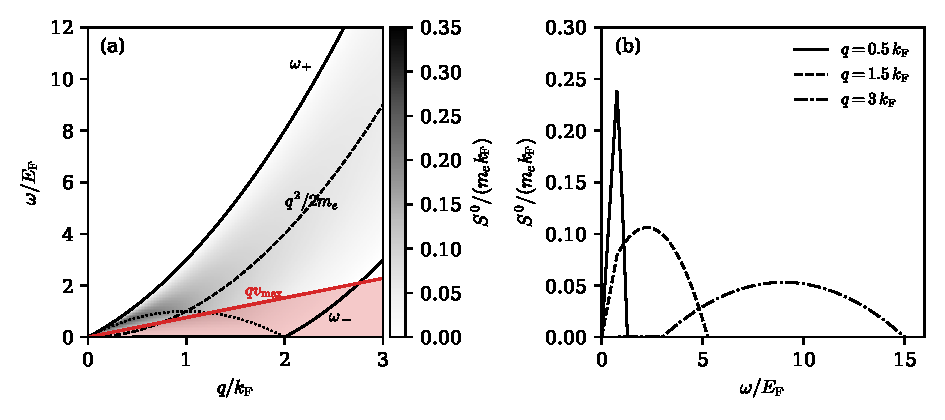
\includegraphics[width=\linewidth]{figures/ch04/fig4_2.pdf}
  \caption{Dynamic structure factor $S^0(q,\omega)$ of the non-interacting electron gas at zero temperature, in units of $m_ek_{\mathrm{F}}$, against the momentum transfer $q$ in units of the Fermi wavevector $k_{\mathrm{F}}$ and the energy $\omega$ in units of the Fermi energy $E_{\mathrm{F}} = k_{\mathrm{F}}^2/2m_e$. (a) Gray scale: $S^0$ inside the particle--hole continuum, bounded above by $\omega_+ = qv_{\mathrm{F}} + q^2/2m_e$ and below by $\omega_- = q^2/2m_e - qv_{\mathrm{F}}$ for $q > 2k_{\mathrm{F}}$ (solid). Below the dotted curve $\omega = qv_{\mathrm{F}} - q^2/2m_e$, $S^0 = m_e^2\omega/\pi q$ grows linearly in $\omega$; above it $S^0$ is a parabola in $\omega$ centered on the free recoil $q^2/2m_e$ (dashed). Red: the energies $\omega \le qv_{\mathrm{max}}$ that dark matter with the maximum halo speed $v_{\mathrm{max}} = 2.65\times10^{-3}$ can deposit, for the valence density of silicon, $\nd_e = \SI{2.00e23}{cm^{-3}}$ ($k_{\mathrm{F}} = \SI{3.57}{keV}$, $E_{\mathrm{F}} = \SI{12.5}{eV}$, $v_{\mathrm{max}} = 0.379\,v_{\mathrm{F}}$). (b) $S^0$ against $\omega$ at $q = 0.5$, 1.5 and $3\,k_{\mathrm{F}}$. At $q = 0.5\,k_{\mathrm{F}}$ the triangle peaks at $0.239\,m_ek_{\mathrm{F}}$ at $\omega = 0.75\,E_{\mathrm{F}}$; at $q = 3\,k_{\mathrm{F}}$ the parabola spans $\omega_- = 3\,E_{\mathrm{F}}$ to $\omega_+ = 15\,E_{\mathrm{F}}$. Every curve integrates to $2\pi\nd_e$ times the fraction of the Fermi sea that can take the momentum $q$, and its first moment is $\pi\nd_eq^2/m_e$.}
  \label{fig:4-gas}
\end{figure}

A gas of atoms is the other independent-particle target, and the one of \cref{sec:2.2}. There the rate off a bound electron was written with single-electron form factors, and the structure factor of a gas of atoms was identified by comparison with the rate formula of \cref{sec:1.5}. The many-body definition now produces it directly.

\begin{workedexample}{Hydrogen from the response matrix}\label{we:4-hydrogen}
Take $N_{\mathrm{at}}$ hydrogen atoms at fixed positions $\vect{R}_\ell$, far enough apart that their wavefunctions do not overlap, in a box of volume $\Vol$, with number density $\nd_T = N_{\mathrm{at}}/\Vol$. At any temperature far below the \SI{10.2}{eV} of the lowest excitation, every atom is in its 1s state. The density operator is a sum over atoms, $n_e(\vect{q}) = \sum_\ell\ee^{\ii\vect{q}\cdot\vect{r}_\ell}$, with $\vect{r}_\ell$ the position of the electron of atom $\ell$. Acting on the ground state it changes one atom at a time. A final state in which atom $\ell$ is in the level $f$ and all others are in 1s is reached by the term of atom $\ell$ alone, with the matrix element $\ee^{\ii\vect{q}\cdot\vect{R}_\ell}f_{1s\to f}(\vect{q})$, since $\vect{r}_\ell = \vect{R}_\ell + \vect{r}$ with $\vect{r}$ measured from the nucleus. The phase drops out of the square, every atom contributes the same, and \cref{eq:4.2-Sab} becomes
\begin{equation}
  S(\vect{q},\omega) = 2\pi\,\nd_T\sum_{f\ne 1s}|f_{1s\to f}(\vect{q})|^2\,\delta(\omega - E_f + E_{1s}) + \frac{2\pi}{\Vol}\,F_{1s}(q)^2\,\Bigl|\sum_\ell\ee^{\ii\vect{q}\cdot\vect{R}_\ell}\Bigr|^2\delta(\omega) ,
  \label{eq:4.2-hydrogen}
\end{equation}
with $F_{1s}$ the elastic form factor \cref{eq:2.2-F1s}. The inelastic term is the structure factor that \cref{sec:2.2} identified by comparing rates. Inserted into \cref{eq:2.5-golden}, it gives
\begin{equation*}
  \varGamma = \nd_T\int\frac{\dd^3q}{(2\pi)^3}\,|\tilde V(\vect{q})|^2\sum_f|f_{1s\to f}(\vect{q})|^2\,2\pi\,\delta(\omega_{\vect{q}} - E_f + E_{1s}) ,
\end{equation*}
which is $\nd_T$ times the $\sigma_Tv$ of one atom, \cref{eq:2.2-bound}. Each atom scatters on its own, and the rate counts atoms; the angle and halo averages of \cref{sec:2.2} then produce the spectrum \cref{eq:2.2-spectrum}. For an atom with several electrons, \cref{eq:4.2-S0} supplies what \cref{sec:2.2} added by hand: the initial orbitals must be occupied and the final ones empty.

The elastic term is where the atoms act together. At a fixed $\vect{q}$ its weight depends on the arrangement of the nuclei. For atoms at random positions the cross terms of $|\sum_\ell\ee^{\ii\vect{q}\cdot\vect{R}_\ell}|^2$ average to zero at $q \ne 0$ and the sum is $N_{\mathrm{at}}$. In a crystal the phases add at the reciprocal-lattice vectors instead. With fixed nuclei the elastic term deposits nothing; free atoms would take up the recoil of the whole atom.

The numbers of \cref{we:2-hydrogen} distribute the weight. At $q = q_0$ the integral of the inelastic term over $\omega$ is $2\pi\nd_T(1 - F_{1s}^2) = 2\pi\nd_T \times 0.59$, of which the $2p$ level takes $0.061$, about a tenth. The elastic term of the random gas carries $2\pi\nd_T \times 0.41$, and by \cref{eq:4.2-static} the two add to $S^{\mathrm{st}}(q_0) = 1$. A gas of independent atoms scatters incoherently at every $q$, and the form factor decides only how much of each scattering excites the atom.
\end{workedexample}

The free gas and the isolated atom are both exact for independent particles, and both miss what makes a solid's response many-body. The f-sum check above is one of a set of exact constraints on $S$ that hold whatever the interactions; \cref{sec:4.3} derives them from causality and commutators, and they are the tests that any computed structure factor of silicon has to pass.
